%Enabling Lazy Shadowing for resiliency in extreme-scale computing 
%brings about a number of challenges and design decisions that need to be addressed, including the applicability of this concept to a large number of 
%tasks executing in parallel, and the runtime mechanisms and 
%communications support to ensure efficient interaction between a 
%main and its shadow.
%In the following, we first introduce the basic Lazy Shadowing resilience model. We then %focus on resilience in extreme-scale computing environments, where a large number of %communicating tasks execute in parallel to complete a job. 
%To achieve high tolerance to failure and reduce energy consumption in these environments, we %propose \emph{Leaping Shadows}, an instance of Lazy Shadowing. The main property of the %leaping shadows resilience model is its ability to sustain forward progress in the presence %of failures.
%. referred to as \emph{leaping shadows}, 
%a technique referred to as \emph{shadowed set rejuvenation} to reduce application failure probability, and 
%\emph{leaping shadows}, 
%as an 
%efficient, forward-progress preserving model to achieve high tolerance to failure, while reducing energy consumption, in these environments. 

 %We also discuss the runtime design issues
%related to enabling runtime support to efficiently achieve 
%the expected levels of resilience in extreme-scale systems. 

%This is to test referring Subsection \ref{frame_single}.



%\subsection{Application characteristics}
%\label{frame_app}
%%\subsection{Computational Model and Assumptions}
We consider the class of tightly-coupled and strongly scaled applications, executing on a large scale computing infrastructure of $N$ cores~\cite{doe_ascr_exascale_2011}. In this framework, the term core represents the unit of computing resource allocation (e.g., a
CPU core, a multi-core CPU, or a cluster node)~\cite{casanova_inria_2012}. This makes our framework agnostic to the granularity of the resource allocation unit.
%The focus of our model is a tightly-coupled and strongly scaling application, which executes on a large-scale platform
%composed of $N$ cores.
%We consider the execution of a tightly-coupled and strongly scaling application, or job, on a large-scale platform
%composed of $N$ cores. The application is tightly-coupled because this is typical in the HPC applications, and strong scaling because weak-scaling applications are not expected to suit for extreme-scale computing of which the cpu/memory imbalance would further increase~\cite{doe_ascr_exascale_2011}. Similar to \cite{casanova_inria_2012}, we use the term core to indicate unit of computing resource allocation (e.g., a
%CPU core, a multi-core CPU, or a cluster node), so that our work is agnostic to the granularity
%of the platform. 
%We assume that a standard checkpointing and roll-back recovery is performed at the
%system level. At most on application process (replica) runs on one core.


The application requires $W$ units of work, and can be split arbitrarily into a set of tasks.
Barriers are used as a method of synchronization among different tasks. Assuming $M \le N$ cores are assigned to the application, the failure-free completion time of the application is $w = W/M$. However, when a core fails, the whole execution will be suspended at the next barrier until recovery is complete. 

%The job can execute on any number $M \le N$ cores. The job is strong scaling so that the time required for a failure-free execution on $M$ cores is $w = W/M$.

%Cores are subject to failures. In most cases, we do not distinguish between soft and hard failures, with the understanding that soft failures are handled via software rejuvenation (i.e., rebooting \cite{466961}) and that hard failures are handled by the replacement of the failed component with a spare, which is a commonplace approach in production systems. For simplicity, we adopt the fail-stop fault model, where a core stops execution once a failure occurs and the failure can be detected by other cores \cite{gartner_faults_1999,cristian_comm_1991}. Since we consider tightly coupled parallel jobs, all $M$ cores operate synchronously. When a core fails, the whole execution is suspended until the failure is recovered. We assume that core failures are independent and identically distributed (i.i.d.). In the real world, instead, failures are bound to be correlated. Obtaining theoretical results for non-i.i.d. failures is beyond the scope of this work. But note that one cause of correlation is the hierarchical structure of computing platforms (each rack comprises compute nodes, each compute node comprises processors, and each processor comprises cores), which leads to simultaneous failures of a group of cores. Our work applies to such failures since a group of failures can be treated as multiple individual failures that happen at the same time and their recovery can be carried out in parallel.

Cores are subject to failures. In our model, we do not distinguish between soft and hard failures. We further assume that soft failures are handled via software rejuvenation (i.e., rebooting \cite{466961}), while hard failures are handled by replacing the failed components with spares. We adopt the fail-stop fault model, whereby a core stops executing upon failure and failures are detected by other non-failing cores \cite{gartner_faults_1999,cristian_comm_1991}. When a core fails, the whole execution is suspended until recovery is complete. 

%%%%%%%%%%%%%%%%%%%%%%%%%%%%%%rethinking%%%%%%%%%%%%%%%%%%%%%%
We assume that core failures are independent and identically distributed (i.i.d.). In the real world, instead, failures are bound to be correlated. Obtaining theoretical results for non-i.i.d. failures is beyond the scope of this work. But note that one cause of correlation is the hierarchical structure of computing platforms (each rack comprises compute nodes, each compute node comprises processors, and each processor comprises cores), which leads to simultaneous failures of a group of cores. Our work applies to such failures since a group of failures can be treated as multiple individual failures that happen at the same time and their recovery can be carried out in parallel.

%Since we consider tightly coupled parallel jobs, all q cores operate syn- chronously. These cores execute the same amount of work W(q) in parallel, chunk by chunk. The total time (on one core) to execute a chunk of dura- tion, or size, ω and then checkpointing it, is ω + C(q)

%\subsection{Leaping Shadows}



%%%%%%%%%%%%%%%%%%%%%%%%%%%%%%%%%%%%%%%%%%%%%%%%%%%%%%%%%%%%%%%%%%%%%%%%%%%%%%%%%%

%%We consider the class of strongly-scaled applications, and use $W$ to denote the size of an application workload~\cite{doe_ascr_exascale_2011}. The workload is split  arbitrarily into a set of $N$ tasks, whose synchronization is achieved using barriers. Assuming that each task is assigned to execute on a core at a maximum speed $\sigma=1$, the failure-free completion time of the application is $w = W/N$. 
Let $M_i$ denote the main process executing the $i^{th}$ task $T_i$, and $S_i$ its associated shadow.
When a failure occurs, the non-failing tasks continue executing until they reach the synchronization barrier. The tasks remain suspended until the shadow associated with the failing task reaches its synchronization barrier.


failure recovery is achieved.  To reduce time to recovery,  we run M shadows simulataneously with the main processes. 
%According to the computational model in Section~\ref{sec:com_model}, an application's workload is split into $M$ parallel tasks where each task is associated with a main process and a shadow.

 The execution of the application can be carried out by simultaneously running all main and shadow processes 
on %$2M$ cores, whereby the main processes execute at the maximum rate while the associated shadows execute at a fraction, $\sigma_s$, of the 
%maximum rate using DVFS. 
%To simultaneously run all the main and shadow processes,
%ne may choose to use $2M$ cores, with $M$ executing the main tasks at the maximum rate and $M$ \emph{lazily} executing the shadows at a fraction, $\sigma_s$, of the 
%maximum rate using DVFS.  
%An alternative method is to use 
$M+S$ cores, where $M$ is a multiple of $S$ and $M+S=N$, all executing at the maximum rate. $M$ of these cores are allocated to the main processes while the remaining $S$ cores are shared among their associated shadows. Based on this method, each main process is allocated one core, while $\alpha=M/S$ shadows are collocated on a single core. $\alpha$ is referred to as the main to shadow ratio.
For example, if $M=9$ and $S=3$, then the 9 shadows execute on 3 cores, with every $\alpha=3$ shadows executing on a core (Figure~\ref{fig:sc_mapping}).
%only $M+S$ cores can be used, whereby the main processes execute on the $M$ cores. And the $M$ shadows are divided into $S$ clusters with of $M/S$ shadows are colocated on a single core, operating at the maximum rate.
%where $M$ is a multiple of $S$, and collocate $M/S$ shadows on each of the $S$ cores, while executing all the cores at the maximum speed. 
%We use $\alpha$ to denote the main to shadow allocation ratio. %, and for simplicity, we assume the maximum execution rate of a core is 1. %Ignoring the overhead of context switching, the two alternatives lead to the same expected execution time, but different power and energy consumption. Specifically, the $2M$-cores scheme consumes more static but less dynamic power/energy than the $M+S$ cores alternative. The ratio between the system static and dynamic power consumption determines which alternative overall consumes less power/energy. 

%In the rest of the paper, we will focus on 
%shadow collocation as the meain the rest of our discussion 
%of the main ideas, concepts and system design. We will assume that all cores in the system execute at maximum speed, with every $\alpha=M/S$ shadows collocated on a core. 
%In HPC, throughput consideration requires that the rate of the main task, $\sigma_m$, and the shadow after failure, $\sigma_a$, be set to the maximum. The execution rate of the shadow before failure, $\sigma_b$, however, may still be used to manage the trade-offs between completion time and energy consumption. Smaller $\sigma_b$ corresponds to lazier shadowing of the main process. 
%In terms of execution rates, this can be expressed as $\sigma_m=\sigma_a=1$ and $\sigma_s \le 1$. 
  
Collocation of $\alpha$ shadows on a core has an important ramification with respect to the resilience of the system. Specifically, to speed up a shadow 
of a failed main to the maximum rate, all other collocated shadows must be terminated. Consequently, a second failure in any of the mains of the terminated shadows cannot be tolerated. In other words, the $M+S$ cores are grouped into $S$ sets, which we call \emph{shadowed sets}, each containing $\alpha+1$ cores with $\alpha$ mains executing on $\alpha$ cores (referred to as main cores) and their corresponding $\alpha$ shadows collocated on one core (referred to as shadow core). Each shadowed set can tolerate a failure in any of its cores, since failure of a main core would be recovered by the shadow core and failure of the shadow core will not affect any mains. After the first failure in a shadowed set, the set is called \emph{vulnerable} because it cannot tolerate another failure. %In the following subsection, we will discuss a rejuvenation scheme that deals with vulnerable shadowed sets.

\begin{figure}[!t]
	\begin{center}
		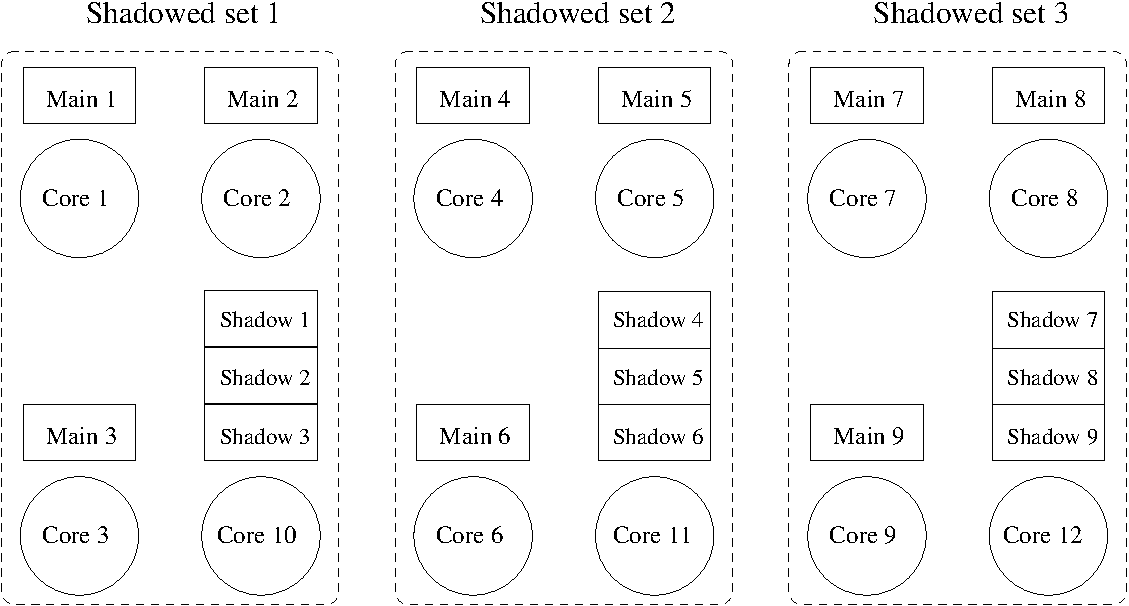
\includegraphics[width=\columnwidth]{Figures/sc_mapping.pdf}
	\end{center}
	\vskip -0.25in 
	\caption{An example of 3 shadowed sets with $\alpha=3$.}
	\label{fig:sc_mapping}
\end{figure}

The lazy shadowing computational model provides the basis for the design of efficient energy- and power-aware fault-tolerance approaches, that takes the energy-delay tradeoffs of the underlying application into consideration. In this section, we show how lazy shadowing can be used as the basic building block for the design of a resilience model for extreme-scale computing environments. The resulting model, referred to as {\it Leaping Shadows}, takes into consideration the main characteristics of tightly-coupled, highly-scalable applications to achieve high-tolerance to failure, while reducing energy consumption, in extreme-scale and failure-prone computing environments. In the following, we first introduce the execution and communication model of the targeted applications. We then describe the dynamics of the {\it Leaping Shadows} resilience model. Lastly, we discuss important aspects of its implementation. 

\subsection {System model}

We consider the class of compute-intensive, strongly-scaled and tightly-coupled applications, executing on a large-scale multi-core computing infrastructure~\cite{doe_ascr_exascale_2011}. Communication between cores is achieved using low-latency, high-bandwidth interconnect networks, such as Infiniband. 

We use $W$ to denote the size of an application workload, and assume that the workload is split  arbitrarily into a set of tasks, $\tau$, which execute in parallel and are synchronized using barriers. Given the prominence of MPI in HPC environments, we assume message passing as the communication model between tasks. Based on this model, each pair of communicating tasks is associated with a logical first-in-first-out  (FIFO) channel, which guarantees ordered delivery of messages.

Assuming that each task is assigned to execute on a core at a maximum speed $\sigma=1$, the failure-free completion time of the application is $w = W/|\tau|$. When a failure occurs, the non-failing tasks continue executing until they reach their synchronization barrier. These tasks remain idle until the failure recovery is complete. The main objective of the Leaping Shadows resilience model is to minimize the idle time induced by failures and ensure forward progress by rolling-forward shadows during the recovery phase. 


%\subsection{Shadow collocation}




\subsection {Leaping Shadows model}

The execution of an application can be carried out by simultaneously running all main and shadow processes for all the tasks. Let $M(i)$ denote the main process executing the $i^{th}$ task $T(i)$ of the application, and $S(i)$ its associated shadow. The task execution is divided into a set of execution phases, each extending over a synchronization interval. In the absence of failure, the behavior of a main  and its leaping shadow is identical to the behavior of a main and its lazy shadow, depicted in Figure \ref{fig:sync}. Figure~\ref{fig:leap} shows the behavior of the main processes and their associated leaping shadows, upon the occurrence of a failure at time $t_f$. Figure~\ref{fig:leap}(a) depicts the execution dynamics of a failing main and its associated shadow. Upon failure of the main process, the associated shadow continues execution, but at a higher rate, until it reaches its synchronization barrier at time $t_r$. 


\begin{figure}[!t]
	\begin{center}
			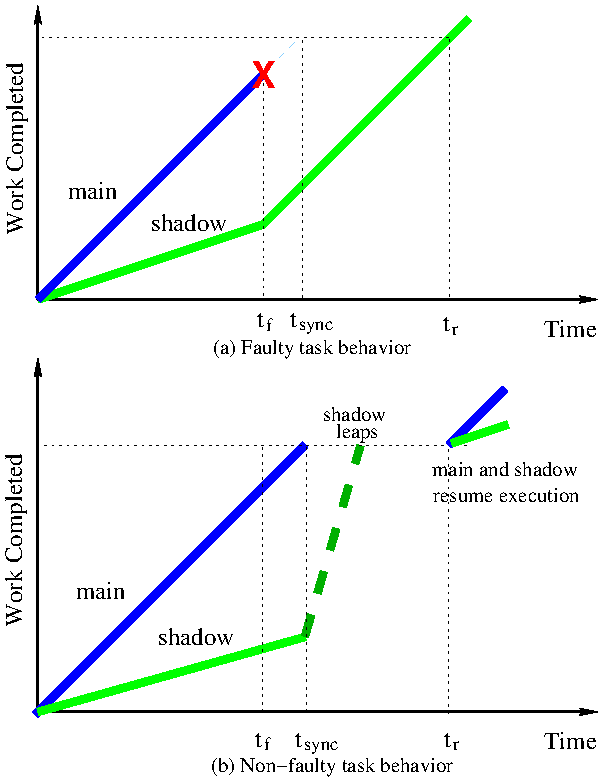
\includegraphics[width=0.8\columnwidth]{Figures/jump.pdf}
	\end{center}
	%\vskip -0.25in
	\caption{The concept of Leaping Shadows.}
	\label{fig:leap}
\end{figure}

Figure~\ref{fig:leap}(b) illustrates the behavior of the remaining main processes and their associated shadows. Unaware of the failed process, the remaining main processes continue executing until they reach their synchronization barriers at time $t_{sync}$. While the shadow of the failed main process progresses toward its synchronization barrier, all remaining main processes become idle until time $t_r$. It is worth noting that, given the tightly-coupled and strongly-scaled nature of the application,  synchronization points occur frequently. Consequently, the time between synchronization points is very small relative to the total execution time of the application. Therefore, if one main, M(i), fails at 
time $t_f$, the remaining main processes will reach their synchronization point, shortly after the failure, specifically at at time $t_{sync} = t_f +\epsilon$, 
where $\epsilon \approxeq 0$. The Leaping Shadows model opportunistically take advantage of the idle time, induced by the failure recovery process, to {\it leap forward} all shadows to their associated non-failing main processes, thereby saving execution time and energy, and guaranteeing forward progress. 
After the shadow of the failing main reaches its synchronization barrier, all processes resume execution from a consistent synchronization point. This process continues until the completion of all tasks. 

Collocation is used to control the leaping shadows execution rates. To execute an application with $M$ tasks, $M+S$ cores are required, where $M$ is a multiple of $S$, all executing at the maximum rate. $M$ of these cores are allocated to the main processes while the remaining $S$ cores are shared among their associated shadows. Each main process is allocated one core, while $\alpha=M/S$ shadows are collocated on a single core. $\alpha$ is referred to as the main to shadow ratio. For example, if $M=9$ and $S=3$, then the 9 shadows execute on 3 cores, with every $\alpha=3$ shadows executing on a core, as shown in Figure~\ref{fig:sc_mapping}.
  
Collocation of $\alpha$ shadows on a core has an important ramification with respect to the resilience of the system. Specifically, to speed up a shadow 
of a failed main to the maximum rate, all other collocated shadows must be terminated. Consequently, a second failure in any of the mains of the terminated shadows cannot be tolerated. In other words, the $M+S$ cores are grouped into $S$ sets, which we call \emph{shadowed sets}, each containing $\alpha+1$ cores with $\alpha$ mains executing on $\alpha$ cores (referred to as main cores) and their corresponding $\alpha$ shadows collocated on one core (referred to as shadow core). Each shadowed set can tolerate a failure in any of its cores, since failure of a main core would be tolerated by the shadow core and failure of the shadow core will not affect any mains. After the first failure in a shadowed set, the set is called \emph{vulnerable} because it cannot tolerate another failure. %In the following subsection, we will discuss a rejuvenation scheme that deals with vulnerable shadowed sets.

\begin{figure}[!t]
  \begin{center}
    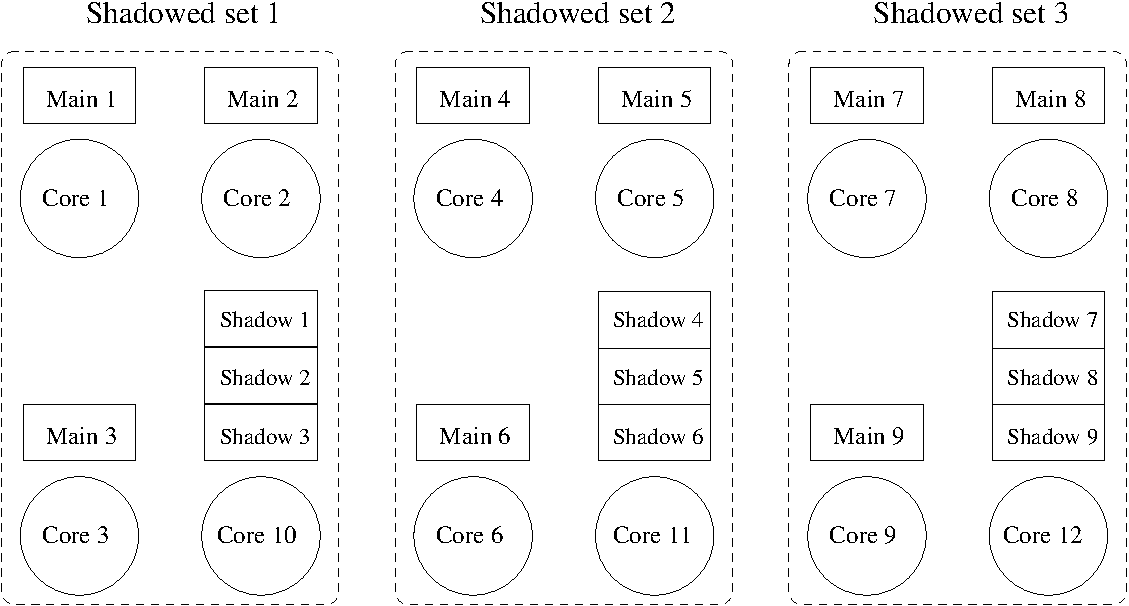
\includegraphics[width=\columnwidth]{Figures/sc_mapping.pdf}
  \end{center}
  %\vskip -0.25in 
  \caption{An example of collocation. $N=12$, $M=9$, $S=3$, and $\alpha=3$.}
  \label{fig:sc_mapping}
\end{figure}





\begin{algorithm}[t]
  \SetKwInOut{Input}{input}
  \SetKwInOut{Output}{output}
  \caption{Lazy Shadowing}
  \Input{$W, M, S$}
  \Output{Application execution status}
  \BlankLine
  split $W$ into $M$ tasks\; \nllabel{line:split} 
  cluster $M$ tasks into $S$ shadowed sets\; \nllabel{line:cluster} 
  %$T_l \leftarrow T+t_{now}$\;%, $C_{vul} \gets 0$
  start M(i) and S(i) for each task T(i)\;
    \While{execution not done}
    {
        \If{failure detected in shadowed set SS(j)} %\nllabel{line:if_start_1} 
        {
            \nllabel{line:if_start_1} 
            \eIf{SS(j) is vulnerable}
            {
                notify ``Application failure"\;
                terminate all mains and shadows\;
                repair all failures\;
                \emph{Restart execution}\; %\Comment{re-execution}
            }
            {
                mark SS(j) as vulnerable\;
                %\State $C_{vul} \gets C_{vul} + 1$
                %\If{$C_{vul} == V$}
                %    \State perform shadowed set rejuvenation   
                %\EndIf 
                \If{failure happened to a main M(k)} 
                {
                    promote S(k) to M(k)\;
                    perform shadow leaping\; %failure induced shadow leaping
                    %$T_l \leftarrow T+t_{now}$\;
                }
            }
        }  
        \nllabel{line:if_end_1}
        %\If{$t_{now} \ge T_l$} %
        %{
        %    \nllabel{line:if_start_2} 
        %    perform shadow leaping\;
        %    $T_l \leftarrow T+t_{now}$\;
        %    \nllabel{line:if_end_2}
        %} % 
        %\nllabel{line:if_end_2}
    }
    output ``Application completes"\;
  \label{al:ls}
\end{algorithm}

The basic steps describing the execution of an application, when using Leaping Shadows based on shadow collocation, are depicted in Algorithm 1.
The total workload is split into $M$ parallel tasks (line~\ref{line:split}). %, which are executed simultaneously by $M$ main processes and $M$ shadow processes. 
To use $M+S$ cores to execute the application, the $M$ tasks are further grouped into $S$ shadowed sets, each with $\alpha=M/S$ cores for $\alpha$ main processes and 1 core for all the associated shadow processes (line 2).  
%The $M$ shadows are then clustered into $S$ groups, each containing $\alpha=M/S$ shadows. 
The execution starts by simultaneously running all the main and shadow processes (line 3).
During the execution of the application,
the system runs a failure monitor that triggers corresponding actions when a failure is detected (line~\ref{line:if_start_1} to~\ref{line:if_end_1}). A failure may trigger different actions, depending on its type and precedence with respect to other failures.  A shadowed set becomes {\it vulnerable} after the occurrence of the first failure. A failure occurring in a vulnerable shadowed set (SS(j)), results in an application failure. In response, the system terminates all running 
processes, initiates a recovery phase, either by rebooting or replacing failing cores,  and restarts execution (line 8 to 10). %(this assumes that checkpointing is not used). 
On the other hand, failure in a non-vulnerable shadowed set
can be overcome through lazy shadowing and does not translate into application failure. In this case, the shadowed set in question (SS(j)) is marked as vulnerable (line 12). Note, however, that a failure in a non-vulnerable shadowed set, can be caused by the failure of a main process or its associated shadow.  While a shadow 
failure does not impact the normal execution of the main processes, and thus can be ignored, failure of the main process forces the remaining main processes to suspend execution after they reach their synchronization point.  The shadow process, S(k), associated with a failing process, M(k),  becomes the primary process of the associated task and increases its execution to the maximum rate (line 14). This, in turn, forces the termination of all other collocated processes.  Simultaneously, a forward leaping process is undertaken by all remaining shadows to align their states with that of their associated mains (line 15).  
This process continues until the application is successfully completed.

\subsection{Leaping Shadows implementation issues}






%\subsection{Shadowed set rejuvenation}
%\label{frame_reju}
%The proposed Lazy Shadowing scheme can tolerate faults which are repairable by rebooting or reconfiguration, referred to as soft faults, and faults which cannot be repaired by rebooting or reconfiguration, referred to as hard 
faults. Monitors that detect hard faults, such as memory flip, bus error 
and latch error, or soft faults, such as deadlock detection, buffer overflow and protection violation, typically interrupt the application to initiate 
the recovery process. The process of recovery from transient or permanent faults is the same and necessitates a mechanism for detecting a fault 
in a main task, M(i) and notifying other tasks in the system so that (i) the shadows sharing a core with S(i) are terminated, thus allowing S(i) to execute at the maximum rate, and (ii) all the shadows that are not in the faulty shadowed set leap to the state of their mains. 

As described earlier, the recovery from a fault in a shadowed set leaves the set vulnerable and any more faults in a vulnerable set will result in a system failure. Although for large systems and small S the probability of having a second fault in a vulnerable set is low, some provision should be taken to rejuvenate the system when a relatively large number of its shadowed sets are vulnerable. 

We propose to invoke \emph{shadowed set rejuvenation} after a specific number of faults, which is determined by the system size, the shadowed set size, and the required resilience.
Rejuvenation reconfigures the system such that none of its shadowed sets are vulnerable. Unlike recovery from a fault in a shadowed set, rejuvenation is different when the faults are transient soft when the faults are hard. In the case of soft faults, rejuvenation can be accomplished by rebooting the failed cores, and restarting the lost shadows (both the ones promoted to mains and the ones terminated) from the state of current mains. And in case of hard faults, it is possible to restart the lost shadows after replacing the failed ones with spare ones. This will restore a vulnerable shadowed set to its original configuration. %For example, rejuvenation should restore the systems shown in Figure~\ref{fig:layout2} and Figure~\ref{fig:layout3} to the one shown in Figure~\ref{fig:layout1}.

%When failures are permanent, rejuvenation may be challenging if rebooting or reconfiguration can no longer be
%used to recover failed components.
%Specifically, in the absence of spare components (if the system is not over-provisioned),
%rejuvenation can only 
%be accomplished by distributing the main processes of a vulnerable set 
%to other {\bf non-vulnerable} shadowed sets. The shadow of the vulnerable 
%set must also be relocated to the shadows of the non-vulnerable set. 
%As a result,  the total number of shadowed sets decreases, but 
%the size of some shadowed sets increases.  In Figure~\ref{fig:reju}, we show a possible rejuvenated configuration assuming that the failure of the cores executing $M(1)$ and $M(14)$ in Figure~\ref{fig:layout2} is permanent. In this restored configuration, the number of shadowed sets is reduced from 8 to 6, with four sets containing three mains each and two sets containing two mains each. Rejuvenating the vulnerable configuration of Figure~\ref{fig:layout3} after a permanent socket failure is more complex but follows the same basic principle.

%\begin{figure*}[ht]
%	\begin{center}
%		\includegraphics[width=\textwidth]{figures/reju.pdf}
%	\end{center}
%\vskip -0.25in
%	\caption{Shadowed set rejuvenation of the vulnerable sets resulting from permanent faults.}
%	\label{fig:reju}
%\end{figure*}


%%%%%%%%%%%%%%%%%%%%%%%%%%%%%%%%%%%%%%%%%%%%%%%%%%%%%%%%%%%%%%%%%%%%%%%%%%%%%%%%%%


State consistency is required both during normal execution and following a failure of a main process to roll-forward the state of the leaping shadows. During normal execution, shadows remain mute, in the sense that 
all outgoing messages from shadows are suppressed. 
A shadow process, however, will typically lag behind its main process during execution. Therefore, it is necessary to ensure that the shadow's state is consistent with that of its associated main, to successfully complete its associated task in case of failure. To this end, a message-logging protocol is used to ensure consistency~\cite{Marz}. These protocols typically use a minimum amount of meta-information to store and replicate the non-deterministic decisions in the execution of an application.  These meta-data, also called determinants, are exchanged through system-level messages. To provide correct recovery after failure, 
a mechanism is required to guarantee that every shadow process follows the same computation and communication steps as its main process. 
After a main process M(i) fails, S(i) will take over M(i)'s role to recover from this failure. If there are other shadows sharing the same core with S(i), they will be terminated and S(i) will start consuming the messages in its receiver-side message log at a faster speed. The message logging protocol will ensure that shadow S(i) reaches a consistent state with the rest of the system. 

Upon failure of a main processes, all shadow processes must update their address space to ``catch up" with their associated non-failing main processes. A technology, such as remote direct memory access (RDMA), to roll-forward the state of the shadow to be consistent with that of its associated main. Rather than copying data to the buffers of the operating system, RDMA enables the network adapter to transfer data directly from the main process to its shadow. The zero-copy networking feature of RDMA considerably reduces latency, thereby enabling fast transfer of data between the main and its shadow.

 


